\documentclass{beamer}

\usepackage{graphicx}

\title{Creaci\'on de un Pipeline de Datos y API con Cach\'e Inteligente}
\author{Jos\'e Roberto Bautista Cubas \\ 20221001417}
\institute{UNAH}
\date{25 de julio del 2025}

\begin{document}

\frame{\titlepage}

\begin{frame}
\frametitle{Link a repositorio de GitHub}
	\url{https://github.com/josejosepreso/api_redis_cache}
\end{frame}

\begin{frame}
\frametitle{Migraci\'on de datos}
	Se utiliz\'o el dataset \url{https://www.kaggle.com/datasets/rishgeeky/indian-pharmaceutical-products}

	\vspace{1em}

	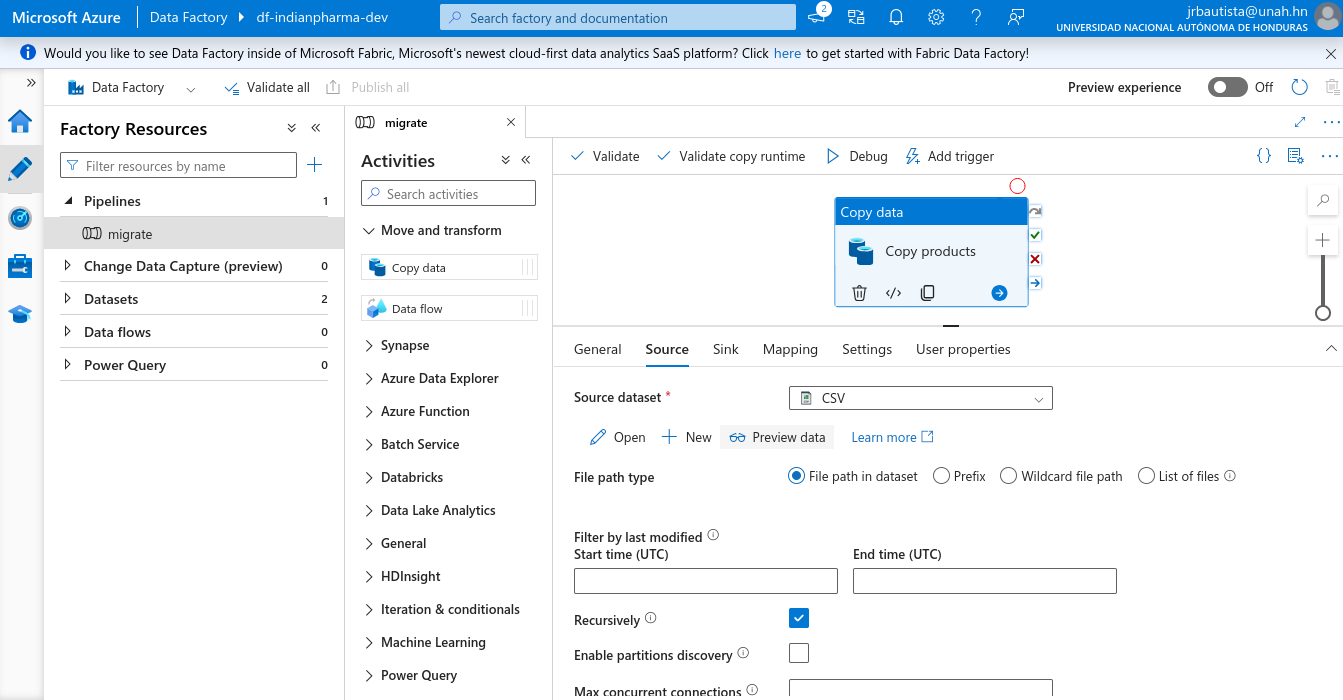
\includegraphics[width=\textwidth]{01.png}
\end{frame}

\begin{frame}
	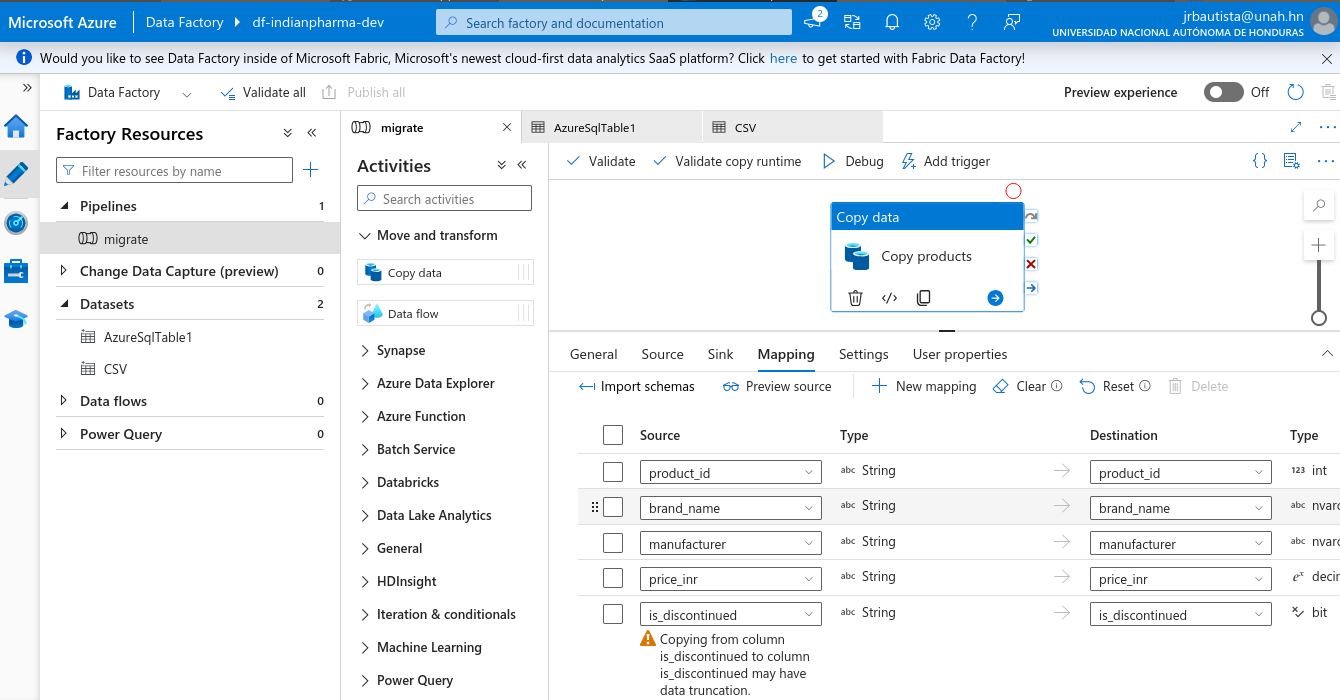
\includegraphics[width=\textwidth]{02.png}
\end{frame}

\begin{frame}
	\frametitle{Application Insights}
	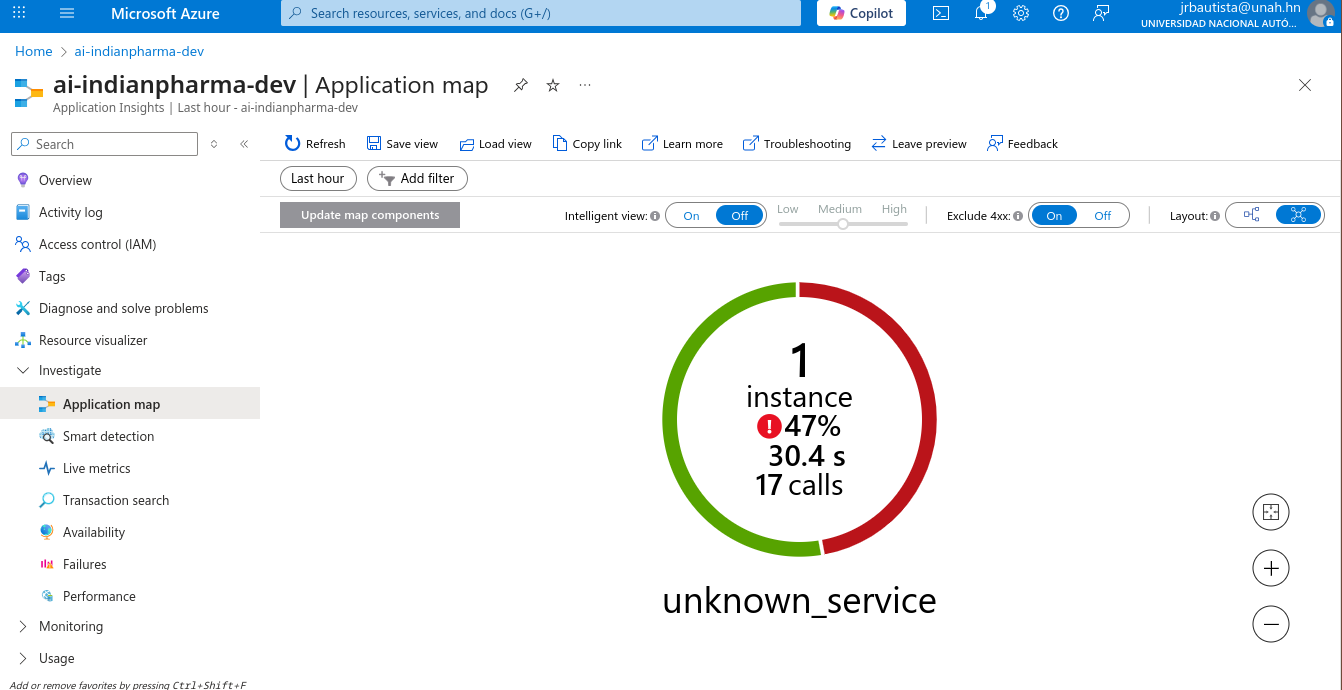
\includegraphics[width=\textwidth]{3.5.png}
\end{frame}

\begin{frame}
	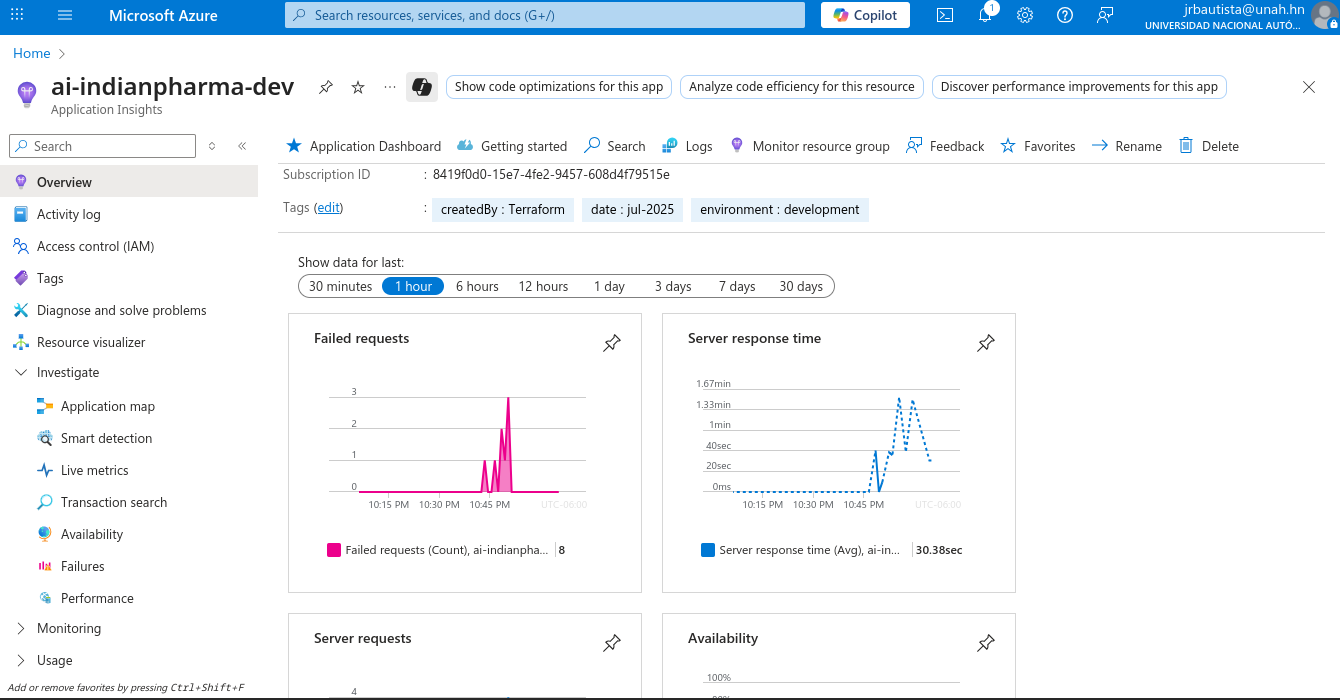
\includegraphics[width=\textwidth]{03.png}
\end{frame}

\begin{frame}
	\frametitle{Despliegue en la nube con Docker}
	
\includegraphics[width=\textwidth]{04.png}
\end{frame}

\end{document}
